\documentclass{article}

\pagestyle{myheadings}

\usepackage{graphicx}
\usepackage{amsmath}

\title{Developing a Better Understanding of the Factors Involved With Facilitating the Movement of Refugees From Their Countries of Origin Into Safe Haven Countries}
\author{\ \ }

\begin{document}

\maketitle

Humanitarian organizations that aim to settle refugees in Europe are currently facing new challenges because refugees are coming from outside Europe in larger numbers than ever before\footnote{http://www.bbc.com/news/world-35091772}. One of these organizations, the office of the United Nations High Commissioner for Refugees (UNHCR) was initially formed in 1950 with the intent to help Europeans displaced by World War II\footnote{http://www.unhcr.org/pages/49c3646cbc.html}. Since its inception the UNHCR has provided aid to refugees, internally dispaced people, stateless people, and asylum seekers from emergencies originating within Europe and, increasingly, outside of Europe.\footnote{http://www.unhcr.org/pages/49c3646cbc.html}.

Conflict and poor governance are seen as the main reasons that people become refugees\footnote{http://www.bbc.com/news/world-35091772}. The 1951 refugee convention defines a refugee as ``owing to a well-founded fear of being persecuted for reasons of race, religion, nationality, membership of a particular social group or political opinion, is outside the country of his nationality, and is unable to, or owing to such fear, is unwilling to avail himself of the protection of that country''\footnote{http://www.unhcr.org/pages/49da0e466.html}, rather than a migrant, who is someone moving from one country to another without refugee status. According to data from the UNCHCR Global Trends 2014, ongoing conflicts in Syria and Afghanistan are the largest source of refugees\footnote{$http://ec.europa.eu/echo/files/aid/countries/factsheets/thematic/refugees_en.pdf$}. When considering how to solve the refugee crisis, it is important to pair dealing with the root causes with safe and efficient relocation of refugees.

Immigrants travel multiple routes -- beginning at the middle east, and travelling through the West, East, and Central Mediterranean, the West Balkans, the Eastern Borders, and from Albania to Greece.
CITE TRAVEL MAP

\begin{center}
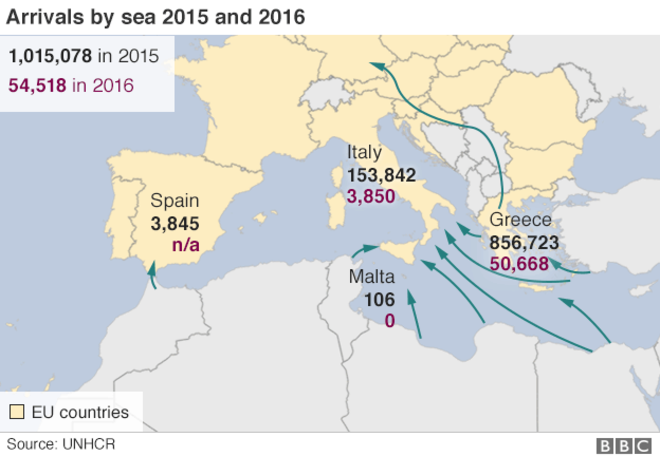
\includegraphics[scale=0.5]{travelmap}
\end{center}

\begin{enumerate}
    \item The majority of refugees resettle in the middle eastern countries of Jordan, Lebanon, and Turkey.
    \item 1,015,078 refugees arrived by sea in 2015.
    \item 942,000 refugees sought asylum in the European Union in 2015\footnote{Eurostat}.
    \item 315,000 have sought asylum in Germany, yet more than 1 million have been counted in Germany's EASY system\footnote{http://www.bbc.com/news/world-europe-34131911}.
    \item 174,055 applied in Hungary.
\end{enumerate}

The political climate surrounding refugee aid in Europe is highly variable and subject to rapid change. Poorly managed camps in Hungary have damaged the reputation of migrants, leading to a surge in the popularity of the radical nationalist Jobbik party\footnote{http://www.bbc.com/news/world-europe-34280460}. The way countries will handle immigration crises cannot be deterministically modeled, so this is considered to be an exogenous factor. In other countries, such as Germany, strong moral foundations protect the influx of immigration\footnote{http://www.bbc.com/news/world-europe-33700624}, with little (and strongly opposed) backlash at the new immigration policies. In addition, unpredicted disasters such as the Paris attacks may threaten refugee relations with their host countries. In November 2015, the incoming Polish Minister for European Affairs said ``we will accept refugees only if we have security guarantees'' \footnote{http://www.bbc.com/news/world-europe-34826438}. The Paris attacks deepened the level of mistrust towards refugees across Europe, since it was believed that the terrorists snuck into the country with refugees. Regardless of the truth of these facts (the only known attackers are French and Belgian residents), the coinciding events were treated as such, and has lead to border problems in the country. Although the only known terrorists were French and Belgian residents, if there is increased mistrust towards refugees that may lead to changes in publically acceptable refugee policy.

We have been tasked with building a model that will help develop a better understanding of the factors involved with facilitating the movement of refugees from their countries of origin into safe haven countries. In doing this, we are attempting to determine the safest and most efficient routes that refugees should take and how many refugees should travel along those routes at a time. The numbers of refugees that should take any given route will relate to the capacity of possible destinations within Europe and the number of refugees within the system. 

Any proposal regarding large volumes of refugee movement should be considered a short term proposal. The resources available for refugee aid are finite, and the impetus for humanitarian aid may decrease over time, causing assumptions that are used to determine optimal travel routes to become inaccurate over longer time periods. The only way to permanantly ease the migrant situation in Europe is to end the conflicts that make people flee their countries in the first place. Therefore, we should only project our models into short time periods in the future.


This problem breaks down into multiple problems.

\begin{enumerate}
    \item {\bf What are the factors involved with moving refugees?}

    The UN asks us to prioritize the health and safety of refugees. What attributes enable or inhibit the safe and efficient movement of refugees? We consider the total numbers of refugees in the system and at each node, entry points for refugees, possible routes, popularity and capacity of those routes, length of routes, mode of transportation along the route, infrastructure for accommodation along routes, and capacity of European countries to recieve refugees to be 

    The total number of refugees entering the system and at each node, the entry points for refugees and capacity of European countries to recieve countries are important variables within the system. The entry points for refugees, possible routes, the popularity and capacity of those routes, the length of routes, mode of transportation and availabilty of infrastructure for accomodation along those routes are parameters to be considere in the system.

    Safety will be optimized by minimizing the risk that any individual may not complete a route. We define a measure of risk that incorporates information about liklihood of illness, death (i.e. drowning on water routes), and other dangers of travel that may be exacerbated for routes with high throughput for a given route. We assume that low densities have low risk and that high densities have high risk. In the absence of data describing this relationship further, for simplicity we assume that population density on a route has a positive linear relationship to risk. If more data becomes available, then a more realistic density-risk function may be substituted into the model.

    To assess the efficiency of a route, one may consider a case with high numbers of migrants to determine where bottlenecks occur and the factors that are slowing down flow at that point on the graph. Efficiency can be incorporated into the selection of an optimal route by favouring shorter routes or including a penalty for slower travel and for long waits in camps before reaching the end destination and exiting the system. Policy that prevents a high number of individuals existing for long periods of time without settling in a country should be preferred.

    Assumptions: All migrants who make it to their destination travel at the average rate. Due to our choice of a linear programming model, all relationships are linear. 

    \item {\bf How do we gain a better understanding of the factors?}

    Create a model of optimal refugee movement, considering accessibility of transport, safety of route, and resource capacities of countries. Use metrics considered to predict the number of refugees that are to be moved, as well as the rate and point of entry necessary to accomodate their movement. Explain new elements you have incorporated into the migration process.

    It should be noted that we must account for dynamically changing environmental factors. Our model should exhibit a use of endogenous change (prepositioning and allocating resources) to form the best route planning approach. Exogenous parameters (unavoidable, unpredictable events, like the terrorist attack in France) must also be considered.

    Graph with connected nodes. Known number of people at a number of entry points. Need to optimize distribution.

    Modelling methods considered:
    Stochastic Differential Equations are used in the stock market because individual factors cannot be influenced. This may be a way to realistically model the randomness of individual refugee movement. However, this type of model is difficult to optimize, which may make it difficult to meet our objective to optimize refugee movement. The use of stochastic programming may allow for optimization of the model. Stochastic effects are generally more important when you are dealing with small population sizes\footnote{Vries {\em et al.} 2006}. Since stochastic effects will likely have little impact on the overall movement of large groups of refugees along major migration routes, it is reasonable to model this situation using deterministic models. 

    Propogater models

    Modelling refugee movement may be treated as a social network problem, with multiple sources and sinks. Travel through the system may be described using fluid dynamics with partial differential equations describing each time step. One way to model exogenous events would be to 

    Create a graph where edges describe travel routes and vertices represent various locations that refugees may travel through and to.

    What do we know about our system?
    How much feedback exists in our system? Is it a closed system? 
    Let us consider a model that describes refugees that are not settled. This includes migrants who are residing in refugee camps in Northern Africa, migrants who are in transit, and migrants who have reached a destination, but do not have accepted migrant status (?) and have not been officially settled in the country. If a migrant becomes officialty settled then they have left the system. 

    Starting with a basic model, each possible country near Europe where there may be a substantial refugee population is represented as a vertex on a graph. The edges between vertices represent the connectivity between locations for refugees. Rates of travel along edges may vary based on qualities of the travel route including capacity, distance, modes of transportation available and risk to migrants. Once these variables and parameters are related on a graph, we need to learn about the dynamics of the system.


    One way to inform the movement of refugees from their country of origin into safe haven countries is to learn about how our system behaves when safety and efficiency are optimized. Safety and efficiency are optimized when risk is minimized and \underline{\ \ \ \ }, respectively. Risk and \underline{\ \ \ \ } can be combined linearly, resulting in an overall measure that determines We chose to use linear programming to optimize our system because it can always be solved. 

    Question?

    \item {\bf Propose a set of policies to the UN}

    Write a report to the UN, proposing a set of policies to enact which will support the conditions for optimal migration (optimal to the UN's views).
\end{enumerate}
\section{Linear Programming}

Our goal is to identify the optimal travel routes for refugees emmigrating for asylum. According to data from the UNCHCR Global Trends 2014, ongoing conflicts in Syria and Afghanistan and other countries in the Middle East and Africa are the largest source of refugees\footnote{$http://ec.europa.eu/echo/files/aid/countries/factsheets/thematic/refugees_en.pdf$}. Many of these refugees flee to neighbouring countries in the Middle East\footnote{$http://ec.europa.eu/echo/files/aid/countries/factsheets/thematic/refugees_en.pdf$}. We are interested in modeling refugee travel from refugee camps, or source nodes, in the Middle East to European countries where the refugees may be integrated into society. It is not economically feasible to move large numbers of refugees across the Atlantic Ocean to North America due to the large distance and travel costs involved, so refugee movement to countries such as Canada and the United States will not be addressed in this model. 

We must optimize the travel routes of refugees for safety and efficiency, under realistic constraints that prevent a utopian immigration process. This is most naturally formed as a linear program. For each route that refugees could travel, we allocate a certain number of refugees. We wish to prevent overcrowding routes and to avoid sending refugees down dangerous routes because an optimal travel route is safe. Safety concerns will be incorporated into our model with a risk parameter. 

Given a country's refugee quota (See Table 1 INSERT TABLE HERE PLEASE) we define that value as the capacity ($C_w$) of any given destination country $w$, or the maximum number of refugees that may settle in that country. The capacity incorporates the fact that there are limited resources available for refugee support in Europe. However, there may be a greater demand for those resources than can be accomodated. More refugees may enter the system than can be accomodated by every destination country even at their maximum capacity. This information can be used to decide which policy decisions should be made in order to organize refugee movement.

We begin by forming a directed graph, summarizing the routes that refugees can take. We consider ach simple path $(v_1, \dots, v_n)$ in the graph because refugees are unlikely to take cyclic routes. For each simple path, we allocate a specific number $x_{(v_1, \dots, v_n)} \in \mathbf{R}$, that represents the number of refugees allocated to that route. ADD ILLUSTRATIVE GRAPH HERE The constraints previously described can be summarized by the following equations

\begin{enumerate}
    \item (No Refugee Left Behind) For every source node $v$, we have
    %
    \[ \sum_{\substack{(v_1, \dots, v_n) \\ v_1 = v}} x_{(v_1, \dots, v_n)} = R_v \]
    %
    Where $R_v$ is the number of refugees exiting the node $v$.

    \item (Every Country is Bounded by its Capacity) For each possible country $w$ in which a refugee may take asylum, we have
    
    %
    \[ \sum_{\substack{(v_1, \dots, v_n) \\ v_n = w}} x_{(v_1, \dots, v_n)} \leq C_w \]
    %
    Where $C_w$ is the capacity of the node $w$.
\end{enumerate}

We formulate risk as a quadratic constraint with multiple factors. First, we take the risk of a route into account. Each edge $(v,w)$ in the graph is associated with a certain `risk constant' $K_{(v,w)}$ that represents the probability of death for a single refugee travelling along that edge. Of course, if $n$ refugees travel along this path, then the expected number of deaths is $n K_{(v,w)}$. The risk of death travelling along a certain path $(v_1, \dots, v_n)$ is then compounded. By basic laws of probability, we have
%
\[ \mathbf{P}(\text{immigrant dies on}\ (v_1, \dots, v_n)) = \sum_{i = 1}^{n-1} \mathbf{P}(\text{immigrant dies on}\ (v_i, v_{i+1})) \]
%
Since the event of dying on a certain interval is obviously independant of dying on a disjoint interval, we have an analogous equation for the constant,
%
\[ K_{(v_1, \dots, v_n)} = \sum_{i = 1}^n \left( \prod_{j = 1}^{i-1} \left(1 - K_{(v_j,v_{j+1})} \right) \right) K_{(v_i, v_{i+1})} \]
%
This expression of risk forms our first linear constraint on the system.

Our second concern is overcrowding. In an overcrowded group factors such as disease and crime are likely to cause harm to travelling refugees, so the density of travellers must be considered. This is a rather simple constant to form. The number of interations within a population of size $n$ is quadratically related to population density. It follows that the risk factors are quadratically related to population density. We assume that there exists a constant $B$ such that the relationship of death rates for $x$ people on a given route is approximated by $Bx^2$. 

Finally, the idea that shorter paths are more optimal needs to be incorporated in to the model. If we have a distance function $d$ on the vertices that provides the length of a route to travel from one vertex to another, then refugees will travel a distance proportional to the sum of the distances of the edges they travel along. Thus we add another constant $C$ relative to the distance traveled by refugees because longer routes are more dangerous.

We have thus formulated enough constraints and costs to form a quadratic program.  The standard form of the optimization problem is detailed below:
%
\begin{align*}
    &\text{min} \left( \sum_{(v_1, \dots, v_n)} K_{(v_1, \dots, v_n)} x_{(v_1, \dots, v_n)} + Cn x_{(v_1, \dots, v_n)} + B x_{(v_1, \dots, v_n)}^2 \right)\\
    &\text{such that, for each source $v$ and sink $w$,}\\
    &\ \ \ \ \ \ \ \ \ \ \ \ \ \ \ \ \ \ \ \ \ \ \ \ \ \ \ \ \ \ \sum_{\substack{(v_1, \dots, v_n) \\ v_1 = v}} x_{(v_1, \dots, v_n)} = R_v\\
    &\ \ \ \ \ \ \ \ \ \ \ \ \ \ \ \ \ \ \ \ \ \ \ \ \ \ \ \ \ \ \sum_{\substack{(v_1, \dots, v_n) \\ v_n = w}} x_{(v_1, \dots, v_n)} \leq C_w
\end{align*}
%
This may be solved via any of your favourite quadratic optimization methods.

\section{Deriving the Path Correlation Coefficient}

Currently, our linear program does not take into account the intersection of paths formed by travelling refugees. Furthermore, it assumes that refugees travel deterministically, not dispersing in response to extraneous events. This obviously does not hold. No two refugees are completely alike, and react differently in response to different events.

The reason why this problem arises when studying the correlation between two different paths arises when two paths intersect. Consider the diagram below, consisting of two curves, with unit speed parameterizations $c$ and $c'$. Suppose that we model the movement of refugees as a single point moving along the line. Then the movement of two groups of refugees coincides when $c(t) = c'(t)$. If the traces of $c$ and $c'$ intersect, but hit the point at different times, then our model would determine that these groups never meet each other. On the other hand, if $c(t) = c(t')$ where $t$ and $t'$ are two time points very far apart, then we would like to consider these two intersections less important than when $t$ and $t'$ are very close. We solve this problem by taking a stochastic movement along these curves.

INSERT IMAGE OF CURVES $c$ AND $c'$ HERE

To accomodate the random motion of immigrating populations along a specific route, we apply the theory of stochastic processes. Begin by making the following assumptions
%
TO DO: ADD MORE JUSTIFICATION FOR ASSUMPTIONS
%
\begin{enumerate}
    \item Every immigrant starts the route at the start point.
    \item The movement of immigrants, as a function of time, is continuous.
    \item The average position of immigrants is linearly proportional to the time elapsed since immigration.
    \item Past movement of a certain immigrant cannot predict future movement. That is, the process of immigration is Markovian.
    \item Relative to the `center of mass' of the population, an immigrants movement is normally distributed, whose standard deviation is linearly proportional to time. This represents a `diffusion' of immigrants over time as they travel to their destination, which converges to the final destination asymptotically.
\end{enumerate}
%
First, we pull back the curve $c$ to its domain $[0,A]$, and extending the definition of $c$ to $[0,\infty)$, by definining $c(A + t) = c(A)$ for $t \geq 0$. We shall place a stochastic process on the interval. With the assumptions above, since $c$ has unit velocity at all time points, we can describe the process $X_t$ which models the movement of immigrants via the stochastic equation
%
\[ X_t = \varepsilon W_t + t \]
%
where $\varepsilon$ is a small constant, and $W_t$ is standard brownian motion. We perform this task for each path, represented by a curve $c$, we construct a process following the equation above. If $X_t$ is such an equation, then $c(X_t)$ gives us a stochastic process on the path in the graph. We wish to measure, in some capacity, the `population correlation' between the stochastic processes $c(X_t)$ and $c'(Y_t)$. We cannot use the probability that two particular instances of the motion meet at a certain time point, since, because continuous processes are nasty -- $\mathbf{P}(c(X_t) = c'(Y_t)) = 0$ for all values. The best we can do is to approximate two populations coinciding; fixing a small $\varepsilon'$, and consider the quantity
%
\[ D_{c,c'} = \int_0^\infty \int_0^1 \mathbf{P}(c'(Y_t) - \varepsilon' < c(X_t) < c'(Y_t) + \varepsilon')\ dY_t\ dt \]
%
Though theoretically an approximation, practically, this method should model situations well in practice. Really, two people can never be in the {\it exact} same location at a particular time, so our model really does model the correct situation, provided we pick $\varepsilon'$ so that `vicinity' is both small enough for two populations to affect one another, and big enough so that the quantity above does not converge to zero. In a particular application of this derivation, we can take two independant motions $X_t$ and $Y_t$ for the same curve $c$, to obtain better density constants for the linear programming formulation.

\section{Metrics of Refugee Crisis}

\begin{center}
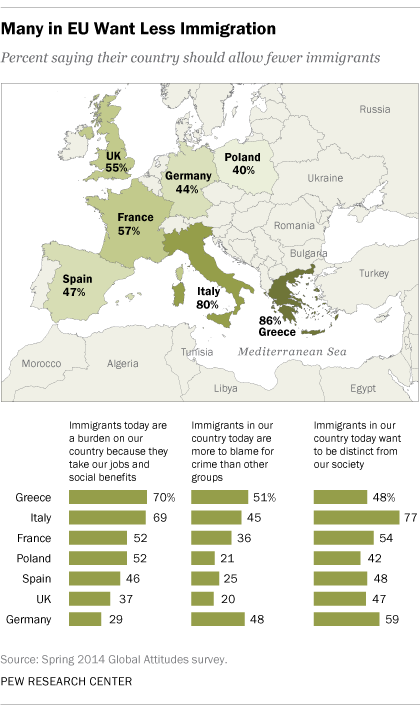
\includegraphics[scale=0.5]{ImmigrationPoll}
\end{center}

\end{document}